One of the first definitions of an \gls{ir} is \emph{``a set of services that a university offers to the members of its community for the management and dissemination of digital materials created by the institution and its community members. It is most essentially an organisational commitment to the stewardship of these digital materials, including long-term preservation where appropriate, as well as organisation and access or distribution. While operational responsibility for these services may reasonably be situated in different organisational units at different universities, an effective institutional repository of necessity represents a collaboration among librarians, information technologists, archives and records managers, faculty, and university administrators and policymakers. At any given point in time, an institutional repository will be supported by a set of information technologies, but a key part of the services that comprise an institutional repository is the management of technological changes, and the migration of digital content from one set of technologies to the next as part of the organisational commitment to providing repository services. An institutional repository is not simply a fixed set of software and hardware.''}\cite{lynch}.

This extensive definition is interesting for a number of reasons. First, it places the repository in the context of an \emph{institution}, an organisation that has \emph{research} as its main object of activity. As a result, it is used for managing \emph{all} outputs that are a result of research; for example, here are three repositories used by universities for managing their scholarship:
\begin{itemize}
    \item DSpace@MIT, the digital repository of the Massachusetts Institute of Technology: \url{https://dspace.mit.edu/}
    \item VTechWorks, the scholarship access platform of Virginia Tech: \url{https://vtechworks.lib.vt.edu/}
    \item ORA, the Oxford University Research Archive: \url{https://ora.ox.ac.uk/}
\end{itemize}

Second, the definition enumerates the three main functions a repository needs to implement:
\begin{enumerate}
    \item Stewardship and organisation: as mentioned in the introduction, repositories are the digital equivalent of physical libraries and, as a result, they need to implement most of the workflows and practices in this area. These include, for example, cataloguing (creating extensive descriptions of the stored content), content classification, or curation.
    \item Preservation: traditionally libraries have ensured that the content they hold remains available over time, and in some cases this requires creating special physical environments necessary for maintaining fragile materials. While digital content might not be afflicted by the exact same issues (e.g., degradation of paper over time), special care is still required in order to ensure that it will remain available in perpetuity. 
    \item Dissemination: scholarship's value increases as the audience it reaches increases; thus it is important that repositories incorporate functionality that will facilitate the distribution and discoverability of content.
\end{enumerate}

As a direct result of the mentioned functions, the definition also mentions that repository staff needs to include not only librarians, but also information technology staff, archivist, researchers, or administrative personnel. In \cite{cmu} the authors describe a repository team comprising of over ten members in three different squads, each serving a different role in the operation of the digital library, from management, to curation, and engagement. Apart from the human resource angle, the repository does not need to be understood as a stand-alone system, but as a collection of modules, each focusing on a specific part of the encompassing workflow and providing a certain functionality to the stakeholders.

Coming back to the presented definition, the most interesting aspect in the context of this work is that it does not explicitly mention the types of content repositories should hold. The author of the cited paper elaborates on this, by making a distinction between \emph{scholarly publishing}, which is concerned, for example, with journal articles or monographs, and \emph{scholarly communication}, which is characterised by the development of new types of output, such as datasets or research software. In fact, scholarly publishing is a subset of scholarly communication, being concerned only with the specific types of outputs characteristic to \emph{traditional} research publishing.

While this definition, including the distinction above, was proposed in 2003, it is important to note that most institutional repositories focus on outputs specific to scholarly publishing (this is also true for the three repositories enumerated above). Nevertheless, the rapid evolution of scholarly communication, fuelled by \gls{oa} and the reproducibility crisis, led to the expansion of the traditional institutional repository in order to allow for the full set of scholarly communication outputs to be part of the managed corpus.

One way to look at this expansion is by considering an intermediate step between traditional institutional repositories and research repositories, namely repositories solely aimed at outputs outside the established publishing model; prime examples are data and research software repositories. Section \ref{sec:data} will take an in-depth look at data repositories while Section \ref{sec:research} will consider how data and institutional repositories merged, creating new systems which aim at managing any scholarly communications output.

\newpage

\section{Data repositories}
\label{sec:data}

Research data repositories have come to prominence as a direct result of the reproducibility crisis, as funders and publishers required researchers to publish all underlying materials along with publications and thus, platforms that could support the new types of outputs were in demand. Apart from the reproducibility crisis, it is worth noting that the scientific endeavour also evolved, researchers producing a wide array of new types of outputs, which traditionally were not published; this means that for a considerable amount of outputs researchers could not receive any credit (review from peers, citations), diminishing the usefulness of the full research activity. An interesting example of such a \gls{ntro} are \emph{negative results} which are generated by experiments, studies or analyses that did not render the expected outcomes; outputs from such endeavours crossed the line between traditional and non-traditional research publishing, as journals dedicated to negative results were established (for example, the Journal of Pharmaceutical Negative Results\footnote{\url{http://www.pnrjournal.com/}}.

As a result, a wide array of data repositories were built, either by non-profit organisations or by private companies capitalising on the new opportunities in the research ecosystem; some examples include:
\begin{itemize}
    \item ZENODO, \url{https://zenodo.org}: a public repository financed by the European Commission
    \item Dryad Digital Repository, \url{https://datadryad.org}: a non-profit repository offering paid curation and preservation services
    \item Figshare, \url{https://figshare.com}: a commercial solution with a free tier for public research
    \item Mendeley Data, \url{https://data.mendeley.com}: a repository solution developed by Elsevier, an academic publisher
    \item PANGAEA, \url{https://pangaea.de}: a data repository targeting the earth and environmental science community
\end{itemize}

As the number of options increased, both researchers and librarians faced the challenge of making the correct choice for publishing research data. This choice depends on a high number of dimensions, spanning both the facilities offered by each repository solution and the legal, policy, and technical requirements of the various stakeholders (researchers, curators funders). A common subset of these can be grouped in three main themes, storage and preservation, metadata, and legal requirements.


\subsection{Data storage and preservation}
\label{subsec:storage}

While data storage has a long history, closely linked to that of computing, research data presents a handful of new and unique challenges, especially when it comes to persistence and privacy. Most often the underlying technology for storing data can be of less relevance for the scholarly and scientific pursuit, but other characteristics can play an important role when choosing a solution.

The first considered aspect is the physical location of the data storage solution. Storing data on a local machine is advantageous as it allows the researcher to quickly access it, but might place obstacles when attempting to share it with a larger team, and also requires that the owner of the machine is fully responsible for its durability. Storage facilities managed at the institutional level, such as \gls{san} systems, move the burden of managing data storage from the individual researcher to specialised personnel, providing higher reliability and enhanced possibilities for sharing data among peers.

Nevertheless, the most common solution nowadays is for data to  be stored off-site in specialised facilities; this model became prominent with the advent of \emph{cloud} systems, such as \gls{aws}, Microsoft Azure or \gls{gcp}, and has benefits in terms of reliability, scalability and accessibility. This might be preferred when the individual researcher or institution does not possess the required resources for managing a storage solution, when large quantities of data need to be stored, or when data needs to be shared across a large network of collaborators. At the same time, the privacy and legal implications need to be considered, given that a 3\textsuperscript{rd} party usually handles the storage. It is worth noting that \emph{cloud} deployments can also be managed by governmental bodies or similar official entities, this alleviating some of the legal issues (for example, the \gls{ands}\footnote{\url{https://www.ands.org.au/}} provides such facilities to researchers in Australia, including storage of sensitive data, such as clinical trial datasets).

From a technical point of view, the choice of a storage solution needs to account for the following:
\begin{itemize}
    \item Redundancy: as no storage system can be guaranteed to function without faults it is important that data is copied and stored on different systems simultaneously. The higher the number of copies and the broader their geographical distribution, the higher the guarantee for their persistence is.
    \item Persistence: simply having data stored on a medium does not provide guarantees that, over time, it would not become inaccessible. For example, both tape drives and hard disks can become demagnetised, hence corrupting the stored data. This phenomenon is frequently described as \emph{bit rot}. Hence, data needs to be periodically tested, and if problems arise, fixed. A common method for detecting issues employs so-called \emph{checksums}, fingerprints of data files which change when even one byte switches value. If a file is detected to have changed it is usually replaced with a redundant copy.
    \item Transformation: as technology evolves, so do the methods for storing data, this also leading to deprecation; for example, floppy disks are rarely used nowadays, despite being ubiquitous just a few years back. Storage and archival systems need to account for this and migrate data to current technological requirements, while ensuring that its contents are not semantically modified.
\end{itemize} 

The second aspect of data storage relates to the employed file formats. While these will most often be enforced by various laboratory instruments and software used for producing and processing data, it is usually beneficial to apply transformations in order to ensure persistence, ease of use, and the possibility for others to work with the data; the decision on formats depends upon multiple considerations.

A first consideration is represented by the choice between proprietary and \emph{open source} file formats. Proprietary formats place a barrier for other collaborators that need to access the data file, as they might require special software or even hardware licences in order to read and modify these; for example, the Microsoft Office formats for storing tabular data (Excel files such as XLS and XLSX), can be opened only by certain applications, while \gls{csv} files can be manipulated by any text editor.

Another point relates to the standardisation of formats; file formats which are backed up by an established standard provide higher guarantees in terms of accessibility and preservation over time, as clear rules on how data is encapsulated and structured are defined. For example, the \gls{dicom} format is the \emph{de facto} method for storing and transmitting medical information; using it guarantees that any systems that implements the standard can fully read the data files. Similarly, the \gls{cdisc}\footnote{\url{https://www.cdisc.org/}} has developed a number of standards encompassing the whole research workflow, such as the \gls{cdash}, which establishes data collection procedures, or the \gls{stdm}, a standard for clinical data organisation and formatting. As a counter-example, the \gls{csv} format does not have complete standards behind it, and thus, particularities can arise at both the structural and semantic levels.
    
Finally, the effects on the research life cycle need to be considered. Producing data files is most often only the first step in the research workflow. Data files will need to be processed, shared with peers, and published alongside other outputs, such as journal articles. While it is highly improbable that data will maintain the same format along the whole cycle (published data rarely includes the whole initial raw dataset), informed choices can aid the process.

The third aspect to be considered relative to research storage choices relates to the overall structure of datasets; for example, while a single file is a more facile method for storing a data set, issues will arise when it grows in size and it needs to be processed or transferred to other systems. Similarly, a large number of files can pose issues with navigating and understanding the structure.

Large dataset instances, especially those exceeding one terabyte, might prove difficult to handle. Consider, for example, the need to transfer such a large file over the network and the possibility that the connection will drop during the operation; most often the transfer will need to be restarted, wasting the effort\footnote{Even over a fiber-optic connection one terabyte of data will require over one hour to transfer.}. In such cases, splitting the dataset might prove to be a better solution, as each smaller file can be transferred individually and independently of the others, network issues requiring only the re-transfer of unsent files. A number of storage systems include an option for so-called \emph{chunked} or \emph{multi-part} file transfers, where the system automatically splits larger files in smaller blocks, allowing these to be transferred independently, in any order, and at any point in time.

In cases where a large number of files constitute a dataset it is important to describe the overall structure such that other applications or users can understand it. Traditionally, \emph{folders} are used for categorising and structuring content, but these can prove ineffective in describing the full organisation, and certain storage systems might not even implement this facility. A common solution to this issue is including separate file(s) describing the structure, usually called \emph{manifests}, along with the actual dataset files. Preferably these would follow a standard structure and semantics, and for this purpose standards such as BagIt\footnote{\url{https://tools.ietf.org/html/draft-kunze-bagit-16}} and \gls{mets}\footnote{\url{https://www.loc.gov/standards/mets/}} have been established. Along with the structural description, these files can also contain technical information (e.g., checksums) that might ease other processes along the scholarly workflow.

An important distinction to consider, especially in the context of research repositories, is the one between storage and preservation. Preservation is a more involved process than simply ensuring that information is stored physically, being also concerned, as already alluded, with maintaining the integrity of the data, transforming it in order to ensure that it can still be consumed in line with the technological and social realities, and providing sufficient information on the data and its context such that new users can understand its purpose. All three points, and especially the latter, rely on \emph{metadata}, which documents various syntactic and semantic aspects of the underlying dataset; the next subsection provides a detailed description.

\newpage

\subsection{Metadata and identifiers}
\label{subsec:metapids}

Storing research data can have many purposes, from facilitating study replication to allowing further hypotheses to be tested. Nevertheless, archiving only the data points, with no information regarding their purpose, provenance or collection method will exponentially decrease their value over time, as both other researchers and the authors of the data will find impossible to reuse them without further information about the syntax and semantics.

Metadata, \emph{data about data}, is the information created, stored and shared in order to describe objects (either physical or digital), facilitating the interaction with said objects for obtaining knowledge\cite{niso}. Metadata can describe various aspects of the underlying data set, and it is often useful to split the various attributes based on their purpose.

\emph{Descriptive} metadata, such as the title, creators of the dataset, or description, is useful for allowing other users find and achieve a basic understanding of the dataset. Often linked to this is the \emph{licencing and rights} metadata that describes the legal ways in which the data can be shared and reused; it includes the copyright statement, rights holder and reuse terms.

\emph{Technical} metadata, which most often includes information on the data files, such as their formats and size, is useful for transferring and processing data across systems and its general management. \emph{Preservation} metadata will often enhance the technical attributes by including information useful for ensuring that data remains accessible and usable, such as the checksum or replica replacement events. Finally, \emph{structural} metadata describes the way in which data files are organised, and their formats.

Given its complexity, producing metadata can become a significant undertaking, its complexity exceeding even that of the underlying data in certain cases. This is one of the reasons for which the standardisation of metadata has become mandatory, this happening at three main levels.

At the structural level, standardisation ensures that on one hand, a minimum set of attributes is always attached to data sets and, on the other, that enough attributes are present for ensuring proper description of any possible artefact, no matter its origin, subject area, or geographical location. Multiple such standards have been developed, from more succinct ones, such as the DataCite Schema\footnote{\url{https://schema.datacite.org/meta/kernel-4.1/}} or \gls{dcmt}\footnote{\url{https://www.dublincore.org/specifications/dublin-core/dcmi-terms/}}, to more extensive, such as MARC21\footnote{\url{https://www.loc.gov/marc/bibliographic/}} or the \gls{cerif}\footnote{\url{https://www.eurocris.org/cerif/main-features-cerif}}. The usage of these standards might vary across subject areas (e.g., the \gls{ddi}\footnote{\url{https://www.ddialliance.org/}} standard is targeted at survey data in social, behavioural, and health sciences) or the main purpose of the metadata (e.g., the \gls{mets} standard emphasises technical, preservation and structural metadata more than the DataCite schema).

At the semantic level, the focus is on ensuring that the language used for describing data observes a controlled variability both inside a research area and across domains. For example, the CRediT vocabulary\footnote{\url{https://casrai.org/credit/}} defines various roles involved in research activities (analyst, investigator, publication author, etc.), \gls{foaf}\footnote{\url{http://xmlns.com/foaf/spec/}} establishes the terminology for describing and linking persons, institutions and other entities, and the \gls{mime}\footnote{\url{https://tools.ietf.org/html/rfc2046}} standard defines the various file formats.

The third point considered from a standardisation point of view involves the formats used for storing and transferring metadata. The \gls{xml}\footnote{\url{https://www.w3.org/XML/}} is one of the most prevalent formats, almost all standards providing a schema and guidance on employing it. The \gls{json}\footnote{\url{https://www.json.org/}} format is also starting to gain traction, both due to its pervasiveness in web services nowadays, and also due to certain initiatives, such as \url{schema.org} which use it as the de facto output format.

One important aspect of metadata, considered by most standards, vocabularies and formats relates to the usage of identifiers. Similar to social security numbers for persons or serial numbers for devices, when it comes to research data the aim of identifiers is to uniquely and \emph{persistently} describe it. This has become a stringent necessity in the age of internet, both due to the requirement to maintain resources accessible for periods of time of the order of years or even decades, no matter the status or location of the system preserving them at any discrete moment, and also due to the necessity of linking various resources across systems. Similar to bit rot, link rot describes the phenomenon of web addresses becoming unavailable over time, for example due to servers going offline. This can pose significant issues for research artefacts, which need to remain available for longer periods of time due to their societal importance; nevertheless, link rot was proven to be pervasive across scholarly resources\cite{sanderson}, As a result, various elements of research data started receiving identifiers, various initiatives and standards becoming available. The importance of the persistence aspect is marked by the use in the community of the \gls{pid} term.

Even before the prevalence of research data sharing, bibliographic records received identifiers, such as \gls{isbn} for books and \gls{issn} for periodicals. For research data, \glspl{ark} and Handles\footnote{\url{http://handle.net/}} are more prevalent, as these mechanisms facilitate issuing new identifiers and thus, are more suited for the larger volume of produced records.

The \gls{doi} system\footnote{\url{https://doi.org}} is quickly emerging as the industry standard; it builds upon the Handle infrastructure, but adds an additional dimension over it, namely \emph{persistence}\cite{doihandle}. At a practical level this is implemented using a number of processes that ensure that an identified object will remain available online (possibly only at the metadata level) even when the original holding server becomes unavailable and the resource needs to be transferred elsewhere. A \gls{doi} is linked to the metadata of the object, and is usually assigned when the object becomes public. The metadata of the object can be updated at any time and, for example, the online address where the object resides, could be updated when the object's location changes; so-called \emph{resolver} applications are in charge of redirecting accesses of the \gls{doi} to the actual address of the underlying object. Note that the \emph{digital} adjective in \gls{doi} refers to the \emph{identifier} and not the \emph{object}; thus, \glspl{doi} can be created for physical objects, such as books, works of art, or laboratory specimens.

A second important dimension of research outputs relates to individual researchers and institutions. ORCiD is currently the most wide-spread identifier for researchers, with over 8 million registrations\footnote{See \url{https://orcid.org}}, while the \gls{isni}\footnote{\url{http://www.isni.org/}} and the Global Research Identifier Database (GRID)\footnote{\url{https://grid.ac}} provide identifiers for research institutions, groups and funding bodies.

Identifiers have been developed for other entities of significant importance in terms of sharing and interoperability. For example, the Protein Data Bank provides identifiers for the proteins, nucleic acids and other complex assemblies\footnote{\url{https://www.rcsb.org/}}, while GenBank\footnote{\url{https://www.ncbi.nlm.nih.gov/genbank/}} indexes genetic sequences using so-called \emph{accession numbers}.

\gls{rrid}\cite{rrid} aim to cover a wider area, providing identifiers for any type of asset used in the scientific pursuit; the current registry includes entities ranging from organisms, cells and antibodies to software applications, databases and even institutions. \glspl{rrid} have been adopted by a considerable number of publishing institutions and are quickly converging towards a community standard.

The complexity of both the semantic and syntactic dimensions of metadata can create significant obstacles in cataloguing, especially in scenarios where researchers, who have most knowledge on the underlying dataset, are not accustomed to library-specific workflows. To overcome this, the community has devised the \gls{fair} principles\cite{fair}, a concise set of recommendations for scientific data management and stewardship which focuses on the \emph{aims} of metadata.

The \gls{fair} principles are one of the first attempts to systematically address the issues around data management and stewardship; they were formulated by a large consortium of research individuals and organisations, and are intended for both data producers and data publishers, targeting the promotion of maximum use and reuse of data. 

\emph{Findability} relates to the possibility of coming across the resource using one of the many internet facilities. This requires that the attached metadata is rich enough (e.g., description or abstract and keywords are crucial for this), that a persistent identifier is associated and included in the metadata, and that all this information is made publicly available on the internet.

\emph{Accesibility} mostly considers the methods through which data can be retrieved. As such, a standard and open protocol, like the ones used over the internet should be employed. Moreover, metadata should always remain available, even when the object ceases to be, in order to provide the continuity of the record; as previously discussed, a \gls{pid} system, like \glspl{doi} can solve this issue.

\emph{Interoperability} considers the ways in which data can be used, processed and analysed across systems, both by human operators and machines. For this, metadata should both \emph{,,use a formal, accessible, shared, and broadly applicable language for knowledge representation''}\cite{fair} and standardised vocabularies; it is interesting to note that the principles become \emph{recursive} here, mandating that vocabularies describing FAIR data sets should themselves follow the same principles.

Moreover, the interoperability guideline requires that metadata contains \emph{qualified} references to other metadata. This is linked with both the persistent and unique identifiers described earlier, but also to the relations between them, the foundation of \emph{Linked Data}, a concept introduced by the inventor of the \gls{www}, Tim Berners-Lee. This concept relies heavily on the \gls{rdf} specification\cite{rdf}, which allows linking pieces of information\footnote{Chapter \ref{ch:rdf} describes RDF in more detail.}. The linked data concept is of utmost importance to the scholarly workflow, as it can provide a wider image over scientific research, as proven by projects such as SciGraph\footnote{\url{https://www.springernature.com/gp/researchers/scigraph}}, which defines over one billion relationships between entities such as journals, institutions, funders or clinical trials, or SCHOLIX\footnote{\url{https://scholix.org}} which links research data to the outputs that reference it.
 
 Finally, the FAIR principles mandate that research data should be \emph{reusable}, facilitating reproducibility. For this, it requires that metadata contains accurate and relevant attributes (e.g., it describes the columns of tabular data) and information about its provenance. Moreover, it touches on certain legal aspects, such as the need for clear and accessible licencing and adherence to \emph{,,domain-relevant community standards''}, such as, for example, the requirements on patient data protection.

\subsection{Legal requirements and constraints}
\label{subsec:legal}

Research data carries a number of legal constraints which are not specific to traditional academic publishing; this is most often due to the complexity inherent in the creation, dissemination and consumption of research data and thus, repositories targeting this type of output need to implement facilities supporting compliance. It is worth noting that most often neither researchers or librarians will possess complete understanding on policy matters, as this requires specific knowledge on various legal aspects and thus, it is important that the repository software provides guidance on these matters. In the following, three broad categories of such constraints are discussed: data anonymisation, legal frameworks and licencing.

Research data anonymisation allows data to be shared whilst preserving the privacy of subjects or other involved parties. Anonymity is not be confused with confidentiality, although the two are linked; anonymity is the process of not disclosing the identity of a research participant, or the author of a particular view or opinion while confidentiality is the process of
not disclosing to other parties opinions or information gathered in the research process\cite{anonrdata}.

The process of anonymising research data requires that key identifiers are changed or masked. An individual's identity can be disclosed from \emph{direct identifiers} such as names or geographic information, or \emph{indirect identifiers} which, when linked with other available data, could identify someone, like occupation or age. Anonymisation should be planned in the early stages of the research venture and considerations for achieveing it should be built in when gaining consent for data sharing. 

One of the challenges of anonymisation is balance; an agressive approach could result in important information being missed or incorrect conclusions being drawn, all the while balancing the potential of re-identification. If the research data is for public release the probability of potential re-identification needs to be low. It may be acceptable for this probability to be higher for private or semi-public datasets as other controls can be put in place\cite{bmjanon}.

This last point alludes to how repositories can approach anonymisation from a technical point of view. For example, in the US the Health Insurance Portability and Accountability Act of 1996 (HIPAA)\footnote{\url{https://www.hhs.gov/hipaa}} directly addresses anonymisation concerns: it requires that systems and repositories that handle such information need to ensure physical, technical and administrative safeguards that meet the obligations laid out in the Act. This means that a repository solution that implements, for example, an \gls{acl} system can easily prevent unauthorised access to raw data and proper review facilities can ensure that only anonymised data becomes available to the wide public.

In terms of legal frameworks, an important point to note is that these vary based on the geographical applicability area; to illustrate this, the following three examples can be considered:

\begin{itemize}
    \item The \gls{eu} \gls{gdpr}: \url{https://www.eugdpr.org/}
    \item The \gls{uk} Data Protection Act: \url{https://www.gov.uk/government/collections/data-protection-act-2018}
    \item The \gls{us} PATRIOT Act: \url{https://www.gov.uk/government/collections/data-protection-act-2018}
\end{itemize}

The \gls{gdpr} came into force on May 25th 2018 and governs the processing (holding or using) of personal data. Although not specifically aimed at research, it contains a number of stipulations which are applicable. First, \gls{gdpr} has a clearer definition of personal data which is that personal data can be used to identify living people. As well as data containing obvious \emph{identifiers}, such as name and date of birth, this can also include genetic, biometric or online data, if unique to an individual. Second, it notes that data is still personal even if it has been pseudonymised (i.e. identifiers are separated from data points) but dataset and identifiers are held by the same organisation.

The \gls{uk} Data Protection Act 1998 and its 2018 update, which was heavily inspired by \gls{gdpr}, applies in Scotland, England, Wales and Northern Ireland and gives individuals rights of access to request copies of their personal data collected by a researcher. It requires that any processors of personal data must comply with eight principles, which make sure that personal data is:

\begin{enumerate}
    \item Fairly and lawfully processed;
    \item Processed for limited purposes;
    \item Adequate, relevant and not excessive;
    \item Accurate and up to date;
    \item Not kept for longer than is necessary;
    \item Processed in line with your rights;
    \item Secure;
    \item Not transferred to other countries without adequate protection.
\end{enumerate}

There are exceptions for personal data collected as part of research: it can be retained indefinitely if needed and can be used for other purposes in some circumstances; in both situations research subjects need to be informed.

The \gls{uk} Data Protection Act also differentiates between personal and sensitive data. Sensitive data includes, but is not limited to, race or ethnic origin, political opinion, religious beliefs, and physical or mental health. Sensitive data can only be processed for research purposes if explicit consent (ideally in writing) has been obtained, the data is in substantial public interest and not causing substantial damage and distress, or if the analysis of racial/ethnic origins is for purpose of equal opportunities monitoring. 

The legal definition of  personal data is complex and is affected by the act's subsequent update in 2018 and \gls{gdpr}, but the simplest and safest definition is of any information about a living, identifiable individual. This is relevant to anonymisation, as if research data is appropriately anonymised then the UK Data Protection act will no longer apply to it.

The PATRIOT Act was signed into law in the \gls{us} of America in 2001. While not specifically aimed at research, it has impact when it comes to data storage, as grants the potential for the US government to have access to data stored by US cloud servers providers. A common misconception is that avoidance of US-located servers solves the issue, which is only partially accurate. This act would, in theory, allow United States judicial authorities and intelligence agencies to request data stored in cloud services outside of the \gls{us}. The police, the judiciary and intelligence agencies are able in one way or another to request information from higher education and research institutions and any other parties concerned. From a legal perspective access to cloud data cannot be denied and \emph{``cloud service providers can give no guarantees in this respect''}\cite{patriot}. In practice, access can take place in one of two ways:

\begin{itemize}
    \item If the cloud service provider is subject to \gls{us} jurisdiction, a request for release of the data can be made directly to the service provider company in the United States.
    \item If the cloud service provider is not subject to \gls{us} jurisdiction, data may be retrieved from the service provider or the institution, or with the assistance of relevant local judicial authorities or intelligence agencies
\end{itemize}

From a technical point of view, this means that research managers need to be concerned with the location repositories used to deploy their software modules, especially those handling physical storage. At the same time, if the repository is not managed by an \gls{us} company it could implement flexible storage facilities that allow researchers to use the best solution from a technical point of view. 

As is the case with any type of scientific output, research data requires a framework upon which sharing, along with proper attribution, can be achieved. What sets data apart from say, journal papers, is that it can be reused in more ways and such, copyright protocols suited for citing research can prove insufficient when considering, for example, the extraction of new hypothesis from existing data sets. This is why new means of licencing and enforcing copyright have either been devised or borrowed from other domains where reuse is common. When data is shared, the original copyright owner usually retains the copyright, but a license can be applied in order to describe how the data can be reused; when no proper licencing terms are applied content cannot be redistributed or reused.

The \gls{cc} suite of licencing options\footnote{\url{https://creativecommons.org/}} is one of the most popular for research data; the model consists of a modular set of clauses which can be aggregated for obtaining licences with varying degrees of freedom in terms of reuse. As such, the CC BY licence allows unrestricted reuse as long as attribution is given to the original authors, while more restrictive options such as CC BY-NC-SA or CC BY-NC-ND disallow either using a different licence for derivative work (SA, \emph{share-alike)}, or no derivatives (ND) at all respectively, with a supplementary clause forbidding the usage of the data for any commercial interest (NC, \emph{no-commercial}).

Apart from these, other licencing options have been devised for more specific use-cases. For example, research software can use one of the deeds commonly employed across the open source software ecosystem, such as the MIT licence\footnote{\url{https://opensource.org/licenses/MIT}} or the \gls{gpl}\footnote{\url{https://www.gnu.org/licenses/gpl-3.0.en.html}}. Another example relates to licences developed by national bodies, in order to ensure better compliance with the regional laws and regulations; such instances include the \gls{eupl}\footnote{\url{https://joinup.ec.europa.eu/collection/eupl}}, or the \gls{ogl}\footnote{\url{http://www.nationalarchives.gov.uk/doc/open-government-licence/version/3/}}. Finally, data can be placed in the public domain, forgoing any copyright or reuse terms; such content can be associated with a notice such as the one provided by \gls{cc} as CC0\footnote{\url{https://creativecommons.org/share-your-work/public-domain/cc0/}}.

While in general researchers should aim for allowing unrestricted use of their data, as also stipulated by the \gls{fair} principles, this is of course not always possible or desirable due to various ethical, regulatory or even technical reasons. In such cases, consulting with personnel specialised in licencing and copyright issues, such as a librarian or lawyer, might be desirable, in order to avoid issues with certain deeds that might place undesirable obstacles on reuse. For example, the no-commercial (NC) clause in the CC suite can disallow the use of data not only by commercial corporations, but also by research institutions generating minimal amounts of revenue\cite{ccbyncndrisks}. Another example relates to so-called \emph{viral} licences, such as \gls{gpl} or the \gls{cc} SA clause, which allow only derivatives licenced under the same exact terms.

Repositories can facilitate licencing in two ways; first they need to be able to support a wide array of options, thus not preventing researchers from selecting the appropriate licence (see Fig. \ref{fig:lic} for an example). Second, facilities explaining in plain language the various deeds can be implemented. GitHub\footnote{\url{https://github.com}}, a repository commonly used for software but which also stores various \glspl{ntro}, offers such a facility at \url{https://choosealicense.com/}; this allows uses to choose the best licencing option by using a process similar to a flow diagram and also summarises the legal text by pinpointing the most important stipulations.

\begin{figure}[ht!]
\centering
  \fbox{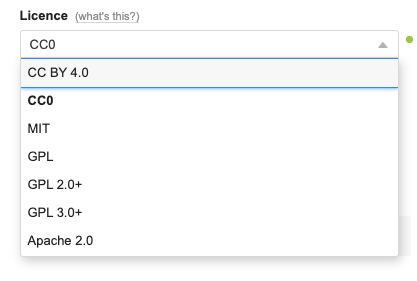
\includegraphics[scale=0.7]{figures/lic.png}}
  \caption{Interface allowing the choice from various licencing options as implemented by the Figshare repository.}
  \label{fig:lic}
\end{figure}

\section{Research repositories}
\label{sec:research}

Data and publication repositories have evolved, at least until recently, as separate platforms; as outlined in the previous section, this was caused in part by the particular features \glspl{ntro} require and, at the same time, by the specific workflows traditional research publishing employs, such as peer review or journal production processes.

Nevertheless, the reproducibility crisis demonstrated the need to have all research outputs available for review at the same time, and having them presented in a consolidated manner can speed up the verification process. From a more technical point of view, this can be accomplished in two manners:
\begin{enumerate}
    \item Develop or employ existing technologies for interlinking research outputs, such as \gls{rdf} or \gls{oai}-\gls{pmh}\footnote{\url{https://www.openarchives.org/pmh/}}.
    \item Aggregate all research outputs on a single repository.
\end{enumerate}

Given the current technology and librarianship space, the first solution is in most cases the most feasible; this is due to the existing infrastructure and the large volume of publications already stored on repositories. To be able to link research outputs in a usable manner, two dimensions need to be considered.

First, researchers need to be able to discern and follow the links; an implementation of this is the mean by which papers and data are frequently linked nowadays. As a result of the new policies around research data sharing, publishers often require authors to upload supporting artefacts to other repositories\cite{elsdat,scidat} and include in articles a statement explaining how they can be accessed; at the same time, the repositories holding \glspl{ntro} can link back to the published article. A full example of this is included in Fig. \ref{fig:link}. This can be facilitated by the use of \glspl{pid}, which, on one hand, distil the linking information in a concise form and, on the other, provide a persistent mean of pointing to the current location of the output, even if the original repository ceased to function and the artefact was transferred elsewhere; this second feature is of utmost importance for physically published media, which is obviously \emph{immutable} and thus, cannot be modified in order to amend links.

\begin{figure}[ht!]
\centering
\begin{subfigure}{0.9\textwidth}
  \fbox{
\includegraphics[width=1\linewidth]{figures/pub.png}}
  \caption{Data accessibility statement linking research article to dataset stored on a specialised repository.}
  \label{subfig:paper2data}
\end{subfigure}
\begin{subfigure}{0.9\textwidth}
  \fbox{
\includegraphics[width=1\linewidth]{figures/dryad.png}}  
  \caption{Reference to the published journal article supported by the dataset which is hosted on the Dryad Digital Repository.}
  \label{subfig:data2paper}
\end{subfigure}
\caption{Bidirectional link between a published journal article and its supporting dataset, source: House et. al. (2020) \emph{Social norms and cultural diversity in the development of third-party punishment}, \texttt{DOI}: 10.1098/rspb.2019.2794.}
\label{fig:link}
\end{figure}

Second, systems that are used to store and disseminate outputs, including but not limited to repositories, need to be able to create, discover and traverse the links between outputs. This is one of the main purposes of the \gls{fair} principles, its importance stemming from the nature of the \gls{www}.

To further emphasise this point, consider the case of \emph{searching} for the study in Fig. \ref{fig:link} using a specialised research search engine. In a naive implementation, such an engine would consider only the metadata of the published paper; this could prove inefficient in cases where the user performs queries pertaining to details of the R\footnote{\url{https://www.r-project.org/}} implementation of the methods used in the study, and which are detailed only in the data package. A search system which is able to understand the link between the paper and the \gls{ntro} could present the user with complete information on the study by providing a consolidated view including both outputs.

Bibliographic metadata is of utmost importance in allowing systems to process links between research outputs. First, metadata needs to include correct and complete information on the artefacts, in order to provide as many opportunities as possible for discovering links between various outputs. Second, as outlined the the \gls{fair} principles, metadata needs to be exposed in a format that promotes interoperability, both at the semantic and syntactic level. Repositories, especially those developed in the early days of the \gls{www}, might struggle with interoperability, as their internal metadata representation did not consider the requirement of allowing other systems to consume it. In Chapter \ref{ch:rdf} a solution for such cases is presented; this solution makes use of \gls{rdf}, this model displaying a series of advantages in terms of linking, as at its core, it implements a knowledge graph.

The second solution to presenting all artefacts pertaining to a research study in the same context revolves around using the same repository for both traditional and non-traditional outputs. In some ways, especially if the distributed nature of the \gls{www} is considered, this can be viewed as counter-intuitive; having each output reside on a platform that best fits its particularities and having them linked as explained above is fully achieving the full potential of the linked \gls{www}.

At the same time, certain realities surrounding the research workflows need to be considered. For example, in a distributed model, researchers might find cumbersome having to upload each output to a different platform, especially if each platform implements the upload process in different manners. In \cite{austin}, the authors note that the amount of time preparing outputs for publishing is a \emph{``major disincentive''} for sharing on repositories, researchers preferring to spend their time on activities which can be credited. Similarly, even in most streamlined linking implementations, consumers of research will still need to follow the various links between outputs and work around the various interfaces repositories employ. Another fact to consider revolves around the administration of repositories; having multiple solutions to maintain can increase the burden on both technology and library resources.

Apart from the consolidation of outputs, using a single repository can provide opportunities for both improving and creating new research workflows. This is best exhibited by the popularisation of new types of outputs, such as:
\begin{itemize}
    \item Pre-registrations: commitment of research plans before executing them, see for example the \emph{``Preregistration Challenge''\footnote{\url{https://osf.io/prereg}}}.
    \item \glspl{dmp}: documents that detail how data will be acquired, managed, analysed and preserved; as these usually describe what repositories will be used,  it seems logical that they are also kept along with the data and other artefacts (for an example see \href{https://doi.org/10.5281/zenodo.1243763}{\texttt{DOI}:10.5281/zenodo.1243763}).
    \item Preprints: while ar$\chi$iv\footnote{\url{https://arxiv.org}}, one of the most well-known \emph{preprint servers} was launched in 1991, preprints came to prominence lately due to their intrinsic property of delivering research results fast, unhindered by traditional publishing practices. For example, during the 2020 \gls{covid} epidemic, over 2000 preprints on the subject have been \emph{posted} on medRxiv\footnote{\url{https://medrxiv.org}} and bioRxiv\footnote{\url{https://biorxiv.org}} between January and April.
\end{itemize}

Three paths to shifting from a specialised repository (e.g., \gls{ir} or data) to a general research repository, able to hold and manage in an meaningful manner any type of research output, can be considered: 
\begin{enumerate}
    \item Develop new features for an existing repository in order to support new types of outputs. For example, Invenio\footnote{\url{https://invenio-software.org/}}, a repository first released in 2002 and developed as an \gls{ir} and library system evolved to be a system which can also hold datasets\cite{invenioabout}, software and other types of outputs, as best demonstrated by ZENODO, which deploys Invenio in its backend. As a reversed route, Figshare, a product that started as a data repository has evolved to also support outputs specific for \glspl{ir}\cite{figntro}.
    \item Migrate existing content to a repository able to manage any kind of outputs. Apart from the opportunity to modernise the repository infrastructure and consolidate administrative, operations or technological resources, this solution might also resolve certain issues generated by commercial, contractual or leadership changes (for an example see the acquisition of Bepress, the developer of the Digital Commons repository\footnote{\url{https://www.bepress.com/products/digital-commons/}}, by Elsevier\cite{bels}). The migration route is further discussed in Chapter \ref{ch:migration}.
    \item Develop distributed repositories: this solution would still consist of multiple systems, each holding various types of outputs, but a single point of entry, for both uploading and consuming content would be provided. In \cite{coar}, the authors make the case for \emph{networked repositories}, in which \emph{}``cross-repository connections are established by introducing bi-directional links as a result of an interaction between resources in different repositories, or by overlay services that consume activity metadata exposed by repositories''. 
\end{enumerate}

While the first two options above are strictly focused on discrete repositories, the third one considers the development of external interoperability frameworks, capable of extracting and providing information from and to the various systems involved in the scholarly workflow. As an example of such infrastructure, Scholix\footnote{\url{https://scholix.org}}, a framework for \emph{``Scholarly Link Exchange''}, currently consists of over 250 million links between research literature and datasets residing in various repositories; any external system can make use of the graph implemented by it in order to present all outputs pertaining to a research study in a consolidated manner. In terms of implementation, Scholix relies on information regarding \emph{associated content} provided by various stakeholders such as repositories, scholarly publishers, or \gls{doi} minting agencies. It is worth noting that the latter can easily become the backbone of such interoperability infrastructure due to the \gls{doi}'s increase in popularity coupled with the requirement for repositories to provide at least minimal metadata for each minted identifier. As such, most agencies provide nowadays the possibility of providing information on known relations between outputs via established relationship types vocabularies\footnote{For an example on how Crossref, a \gls{doi} minting agency, implements this see the \emph{``Relationships between different research objects''} section at \url{https://www.crossref.org/education/content-registration/structural-metadata/\#00040}.}.

Despite the mean of achieving it not being concrete, the vision of research repositories that encompass the plethora of outputs available nowadays is both clear and widely accepted in the community. In \cite{salo}, the author argues that \glspl{ir} should look beyond literature, as otherwise a repository will not fully justify its existence. Even by coming back to the definition in \cite{lynch}, it can be seen that \glspl{ir} were never meant to be limited to certain types of content, mostly peer-reviewed scientific literature, but to cater to any needs the researchers, their workflows and the current societal circumstances call for. Thus, it is important to look at the various options of achieving this vision and let the stakeholders in the scientific endeavour decide which is the best to employ. In the next chapters, original research on certain features that could be implemented in research repositories is presented; the common theme among these is the adaption of techniques specific to software engineering and of technologies employed in other types of applications in the last few decades to the area of digital libraries, touching on all paths presented above, which could lead to a new generation of research repositories.

\newpage

\section{Open Source repositories}
\label{sec:os}

While open science is a relatively new movement, the world of librarianship always took a more \emph{public} approach to the services it delivers, in line with the philosophy that knowledge should be shared freely both across the research community and society as a whole; an interesting effect of this is the development of multiple open source repository solutions.

DSpace\footnote{\url{https://duraspace.org/dspace/}} was first released in 2002 as a solution for the submission, management and preservation of digital records. It features a web interface, a backend written in the Java\footnote{\url{https://www.java.com/}} programming language, a relational database for holding metadata, and a search engine. DSpace uses \gls{dcmt} as its default metadata schema, and includes facilities for \gls{doi} minting, record versioning, and exports via \gls{oai}-\gls{pmh}. DSpace is the most popular repository solution, with almost $2000$ instances recorded on the \gls{roar}\footnote{\url{http://roar.eprints.org/}}.

EPrints\footnote{\url{https://www.eprints.org/}} is considered to be the first digital repository solution, with the initial release in 2000 and with almost 700 instances registered in \gls{roar}. It features both a web and a command line interface and is written in the Perl\footnote{\url{https://www.perl.org/}} programming language. Metadata is stored in a relational database using an internal hierarchical model. The architecture of EPrints is based on \emph{plugins}, which allows customising any functional aspect of the repository.

Fedora\footnote{Not to be confused with the Linux distribution sponsored by Red Hat Inc.} (Flexible Extensible Digital Object Repository Architecture) Commons\footnote{\url{https://duraspace.org/fedora/}} is a digital asset management system which can be used as the foundation of other repositories, from which Samvera\footnote{\url{https://samvera.org/}} (previously known as Hydra) and Islandora\footnote{\url{https://islandora.ca/}} are the most popular. With the first public release dating to 2004, Fedora distinguishes itself by its flexibility, which results from two architectural features. First, it allows seamless conversions from its data model to \gls{rdf}, which enable the usage of any metadata vocabulary for describing bibliographic records and the \emph{linkage} of information residing on external systems; the benefits of \gls{rdf} will be further discussed in Chapter \ref{ch:rdf}. Second, Fedora opts for a service-based design, which allows plugging in any new modules via \gls{rest} \glspl{api}, while ensuring that these conform to the business logic rules of the core system. Fedora is implemented using the Java programming language and uses relational databases for holding metadata records.

Invenio is a software suite which allows running an online, large-scale document repository or digital library. Its features cover all aspects of such repositories, including document ingestion, classification, ranking, indexing, curation and dissemination\cite{kaplun, glauner}; the architecture of the software is highly modular, each component being in charge of one the mentioned aspects or other additional features. Currently, it is being developed by an international developer community and is released as open source software under the second version of \gls{gpl}. The software platform is built using the Python programming language uses a relational database for metadata. Records are represented internally using an \gls{xml} derivative of the MARC 21\footnote{\url{https://www.loc.gov/marc/bibliographic/}} bibliographic format, which is widely used for the representation and exchange of bibliographic, authority, holdings, classification, and community information data in machine-readable form.

While the projects presented up to this point focused mainly on delivering \gls{ir} solutions, Dataverse\footnote{\url{https://dataverse.org/}} is a repository system that treats data as a first-class citizen. Thus, it has aligned its development roadmap with the \gls{fair} principles, including features such as \gls{doi} minting, machine-readable metadata embedded in dataset landing pages, interoperability with external metadata sources, and facilities for licencing and controlling access to datasets. Dataverse also focuses on facilitating and capturing data citations, adhering to the philosphy that \glspl{ntro} can also make an impact in research. Also different from the other reposiroty solutions are the means through with Dataverse can store and present to users complex file formats and non-trivial directory structures. The repository is implemented in the Java programming language and stores metadata in a relational database.

An important aspect shared by all the mentioned repository projects relates to their governance; the development of these solutions is steered by panels of users and experts in the fields of librarianship or information management, in order to ensure that the deliverables are always aligned to the requirements of the research community. For example, at the time of this work, 16 out of the 21 memebers of DSpace's leadership group were affiliated with academic institutions\cite{dspacelead}. Similarly, the Invenio project originated in the world of high-energy physics, being used in production by both the European Organisation for Nuclear Research (CERN) Document Server (CDS), and the INSPIRE repository which is curated by a collaboration of scientist from the Deutsches Elektronen-Synchrotron (DESY), Fermi National Accelerator Laboratory (FNAL), and SLAC National Accelerator Laboratory.

These communities play a crucial role in the development of all repository solutions, not only the open source ones, as they most often define the principles all digital libraries should adhere to. As a result of direct competition, commercial repository vendors must implement the functionalities present in their open source counterparts, this ensuring that the same level of service quality is offered to institutions and researchers that do not possess the technical or administrative resources to deploy a stand-alone repository.